\section[Проектирование программного модуля]{%
  ПРОЕКТИРОВАНИЕ ПРОГРАММНОГО МОДУЛЯ
}\label{sec:design}

В подразделе~\ref{subsec:system_spec_task} было дано простейшее
описание требований к разрабатываемому приложению с точки зрения пользователя.
Целью данного раздела является уточнение требований к мобильному приложению,
разработка его структуры, а также описание различных приемов,
использованных в процессе его проектирования.

\subsection{Общая характеристика задачи}

Проектирование является неотъемлемой частью жизненного цикла
разработки программного обеспечения.
Существует множество различных методологий проектирования.
Каждая из них предполагает описание требований к разрабатываемой системе
и собственно разработку структуры системы, которая им удовлетворяет.
В ходе проектирования требования к системе многократно дополняются и уточняются.
Характер процесса проектирования определятся используемой
методологией разработки программного обеспечения.
На данный момент существует две основные разновидности методологии разработки ПО:
каскадная и итеративная, представленные на рисунке~\ref{fig:design_methods}.

\begin{figure}[h!]
  \centering
  \fcolorbox{gray}{white}{
    {\small
      % Graphic for TeX using PGF
% Title: /home/budnyjj/univer/GIT/diploma/b/design/diagrams/design_methods.dia
% Creator: Dia v0.97.3
% CreationDate: Sun May  8 16:47:35 2016
% For: budnyjj
% \usepackage{tikz}
% The following commands are not supported in PSTricks at present
% We define them conditionally, so when they are implemented,
% this pgf file will use them.
\ifx\du\undefined
  \newlength{\du}
\fi
\setlength{\du}{15\unitlength}
\begin{tikzpicture}
\pgftransformxscale{1.000000}
\pgftransformyscale{-1.000000}
\definecolor{dialinecolor}{rgb}{0.000000, 0.000000, 0.000000}
\pgfsetstrokecolor{dialinecolor}
\definecolor{dialinecolor}{rgb}{1.000000, 1.000000, 1.000000}
\pgfsetfillcolor{dialinecolor}
\definecolor{dialinecolor}{rgb}{1.000000, 1.000000, 1.000000}
\pgfsetfillcolor{dialinecolor}
\fill (20.142500\du,12.182961\du)--(20.142500\du,17.246294\du)--(27.160000\du,17.246294\du)--(27.160000\du,12.182961\du)--cycle;
\pgfsetlinewidth{0.100000\du}
\pgfsetdash{}{0pt}
\pgfsetdash{}{0pt}
\pgfsetmiterjoin
\definecolor{dialinecolor}{rgb}{0.000000, 0.000000, 0.000000}
\pgfsetstrokecolor{dialinecolor}
\draw (20.142500\du,12.182961\du)--(20.142500\du,17.246294\du)--(27.160000\du,17.246294\du)--(27.160000\du,12.182961\du)--cycle;
% setfont left to latex
\definecolor{dialinecolor}{rgb}{0.000000, 0.000000, 0.000000}
\pgfsetstrokecolor{dialinecolor}
\node at (23.651250\du,14.459350\du){Анализ };
% setfont left to latex
\definecolor{dialinecolor}{rgb}{0.000000, 0.000000, 0.000000}
\pgfsetstrokecolor{dialinecolor}
\node at (23.651250\du,15.447127\du){требований};
\definecolor{dialinecolor}{rgb}{1.000000, 1.000000, 1.000000}
\pgfsetfillcolor{dialinecolor}
\fill (19.115000\du,18.814901\du)--(19.115000\du,21.902679\du)--(28.187500\du,21.902679\du)--(28.187500\du,18.814901\du)--cycle;
\pgfsetlinewidth{0.100000\du}
\pgfsetdash{}{0pt}
\pgfsetdash{}{0pt}
\pgfsetmiterjoin
\definecolor{dialinecolor}{rgb}{0.000000, 0.000000, 0.000000}
\pgfsetstrokecolor{dialinecolor}
\draw (19.115000\du,18.814901\du)--(19.115000\du,21.902679\du)--(28.187500\du,21.902679\du)--(28.187500\du,18.814901\du)--cycle;
% setfont left to latex
\definecolor{dialinecolor}{rgb}{0.000000, 0.000000, 0.000000}
\pgfsetstrokecolor{dialinecolor}
\node at (23.651250\du,20.597401\du){Проектирование};
% setfont left to latex
\definecolor{dialinecolor}{rgb}{0.000000, 0.000000, 0.000000}
\pgfsetstrokecolor{dialinecolor}
\node[anchor=west] at (23.651250\du,21.091290\du){};
\definecolor{dialinecolor}{rgb}{1.000000, 1.000000, 1.000000}
\pgfsetfillcolor{dialinecolor}
\fill (20.218750\du,24.728119\du)--(20.218750\du,27.815897\du)--(27.083750\du,27.815897\du)--(27.083750\du,24.728119\du)--cycle;
\pgfsetlinewidth{0.100000\du}
\pgfsetdash{}{0pt}
\pgfsetdash{}{0pt}
\pgfsetmiterjoin
\definecolor{dialinecolor}{rgb}{0.000000, 0.000000, 0.000000}
\pgfsetstrokecolor{dialinecolor}
\draw (20.218750\du,24.728119\du)--(20.218750\du,27.815897\du)--(27.083750\du,27.815897\du)--(27.083750\du,24.728119\du)--cycle;
% setfont left to latex
\definecolor{dialinecolor}{rgb}{0.000000, 0.000000, 0.000000}
\pgfsetstrokecolor{dialinecolor}
\node at (23.651250\du,26.510619\du){Разработка};
% setfont left to latex
\definecolor{dialinecolor}{rgb}{0.000000, 0.000000, 0.000000}
\pgfsetstrokecolor{dialinecolor}
\node[anchor=west] at (23.651250\du,22.635179\du){};
\definecolor{dialinecolor}{rgb}{1.000000, 1.000000, 1.000000}
\pgfsetfillcolor{dialinecolor}
\fill (19.685000\du,29.721535\du)--(19.685000\du,32.809313\du)--(27.617500\du,32.809313\du)--(27.617500\du,29.721535\du)--cycle;
\pgfsetlinewidth{0.100000\du}
\pgfsetdash{}{0pt}
\pgfsetdash{}{0pt}
\pgfsetmiterjoin
\definecolor{dialinecolor}{rgb}{0.000000, 0.000000, 0.000000}
\pgfsetstrokecolor{dialinecolor}
\draw (19.685000\du,29.721535\du)--(19.685000\du,32.809313\du)--(27.617500\du,32.809313\du)--(27.617500\du,29.721535\du)--cycle;
% setfont left to latex
\definecolor{dialinecolor}{rgb}{0.000000, 0.000000, 0.000000}
\pgfsetstrokecolor{dialinecolor}
\node at (23.651250\du,31.504035\du){Тестирование};
% setfont left to latex
\definecolor{dialinecolor}{rgb}{0.000000, 0.000000, 0.000000}
\pgfsetstrokecolor{dialinecolor}
\node[anchor=west] at (29.100000\du,28.598397\du){};
\definecolor{dialinecolor}{rgb}{1.000000, 1.000000, 1.000000}
\pgfsetfillcolor{dialinecolor}
\fill (19.830000\du,33.796008\du)--(19.830000\du,37.871563\du)--(27.472500\du,37.871563\du)--(27.472500\du,33.796008\du)--cycle;
\pgfsetlinewidth{0.100000\du}
\pgfsetdash{}{0pt}
\pgfsetdash{}{0pt}
\pgfsetmiterjoin
\definecolor{dialinecolor}{rgb}{0.000000, 0.000000, 0.000000}
\pgfsetstrokecolor{dialinecolor}
\draw (19.830000\du,33.796008\du)--(19.830000\du,37.871563\du)--(27.472500\du,37.871563\du)--(27.472500\du,33.796008\du)--cycle;
% setfont left to latex
\definecolor{dialinecolor}{rgb}{0.000000, 0.000000, 0.000000}
\pgfsetstrokecolor{dialinecolor}
\node at (23.651250\du,35.578508\du){Техническая };
% setfont left to latex
\definecolor{dialinecolor}{rgb}{0.000000, 0.000000, 0.000000}
\pgfsetstrokecolor{dialinecolor}
\node at (23.651250\du,36.566285\du){поддержка};
\pgfsetlinewidth{0.100000\du}
\pgfsetdash{}{0pt}
\pgfsetdash{}{0pt}
\pgfsetbuttcap
{
\definecolor{dialinecolor}{rgb}{0.000000, 0.000000, 0.000000}
\pgfsetfillcolor{dialinecolor}
% was here!!!
\pgfsetarrowsend{stealth}
\definecolor{dialinecolor}{rgb}{0.000000, 0.000000, 0.000000}
\pgfsetstrokecolor{dialinecolor}
\draw (23.681345\du,11.498039\du)--(23.651250\du,12.182961\du);
}
\pgfsetlinewidth{0.100000\du}
\pgfsetdash{}{0pt}
\pgfsetdash{}{0pt}
\pgfsetbuttcap
{
\definecolor{dialinecolor}{rgb}{0.000000, 0.000000, 0.000000}
\pgfsetfillcolor{dialinecolor}
% was here!!!
\pgfsetarrowsend{stealth}
\definecolor{dialinecolor}{rgb}{0.000000, 0.000000, 0.000000}
\pgfsetstrokecolor{dialinecolor}
\draw (23.651250\du,17.295564\du)--(23.651250\du,18.765168\du);
}
\pgfsetlinewidth{0.100000\du}
\pgfsetdash{}{0pt}
\pgfsetdash{}{0pt}
\pgfsetbuttcap
{
\definecolor{dialinecolor}{rgb}{0.000000, 0.000000, 0.000000}
\pgfsetfillcolor{dialinecolor}
% was here!!!
\pgfsetarrowsend{stealth}
\definecolor{dialinecolor}{rgb}{0.000000, 0.000000, 0.000000}
\pgfsetstrokecolor{dialinecolor}
\draw (23.651250\du,21.952948\du)--(23.651250\du,24.677850\du);
}
\pgfsetlinewidth{0.100000\du}
\pgfsetdash{}{0pt}
\pgfsetdash{}{0pt}
\pgfsetbuttcap
{
\definecolor{dialinecolor}{rgb}{0.000000, 0.000000, 0.000000}
\pgfsetfillcolor{dialinecolor}
% was here!!!
\pgfsetarrowsend{stealth}
\definecolor{dialinecolor}{rgb}{0.000000, 0.000000, 0.000000}
\pgfsetstrokecolor{dialinecolor}
\draw (23.651250\du,27.864147\du)--(23.651250\du,29.673285\du);
}
\pgfsetlinewidth{0.100000\du}
\pgfsetdash{}{0pt}
\pgfsetdash{}{0pt}
\pgfsetbuttcap
{
\definecolor{dialinecolor}{rgb}{0.000000, 0.000000, 0.000000}
\pgfsetfillcolor{dialinecolor}
% was here!!!
\pgfsetarrowsend{stealth}
\definecolor{dialinecolor}{rgb}{0.000000, 0.000000, 0.000000}
\pgfsetstrokecolor{dialinecolor}
\draw (23.651250\du,32.859499\du)--(23.651250\du,33.754824\du);
}
\pgfsetlinewidth{0.100000\du}
\pgfsetdash{}{0pt}
\pgfsetdash{}{0pt}
\pgfsetbuttcap
{
\definecolor{dialinecolor}{rgb}{0.000000, 0.000000, 0.000000}
\pgfsetfillcolor{dialinecolor}
% was here!!!
\pgfsetarrowsend{stealth}
\definecolor{dialinecolor}{rgb}{0.000000, 0.000000, 0.000000}
\pgfsetstrokecolor{dialinecolor}
\draw (23.632448\du,37.921645\du)--(23.626443\du,38.588455\du);
}
% setfont left to latex
\definecolor{dialinecolor}{rgb}{0.000000, 0.000000, 0.000000}
\pgfsetstrokecolor{dialinecolor}
\node[anchor=west] at (23.651250\du,14.714627\du){};
\end{tikzpicture}

    }
  }
  \caption{Методологии разработки программного обеспечения}
  \label{fig:design_methods}
\end{figure}

Каскадная методологии разработки ПО сводится к последовательному
прохождению набора фаз разработки:
анализа требований, проектирования, реализации, тестирования, интеграции и поддержки.
При использовании данной методологии проектирование производится
лишь один раз. Входными данными являются требования к продукту,
а результатом --- набор технических документов, детально описывающих
разрабатываемую систему.
Дальнейшие этапы разработки производятся в строгом соответствии с этими документами;
изменение их содержания на последующих этапах не приветствуется.

Итеративная методология рассматривает процесс разработки ПО как
циклическое прохождение описанных выше фаз разработки.
Это позволяет команде разработчиков более динамично реагировать
как на внутренние, так и на внешние изменения условий и требований.
При использовании данной методологии проектирование производится несколько раз.
На первых порах разрабатывается высокоуровневая архитектура системы,
определяются ключевые требования к ней. Далее, по мере повторения цикла
разработки, производится описание разрабатываемых подсистем и и связей между ними.

Данный проект будет разрабатываться с использованием итеративной методологии:
сначала будет выполнено высокоуровневое описание частей проекта,
а затем по мере реализации уточняются детали функционирования его подсистем.
Проектирование будет выполняться с использованием языка графического
моделирования UML~\cite{fowler04}, а также набора документированных решений,
известных как паттерны проектирования GoF~\cite{gamma01}.

Объектом проектирования является мобильное приложение,
которое представляет собой самостоятельный программный модуль.
Поскольку необходимость интеграции в какую-либо существующую
систему отсутствует, задача проектирования значительно упрощается.
С другой стороны, целевая мобильная платформа выдвигает ряд дополнительных
требований к объекту проектирования:
\begin{itemize}
\item более строгие ограничения на используемые ресурсы;
\item учет разнообразия конфигураций мобильных устройств;
\item поддержка совместимости между различными версиями
  мобильной платформы.
\end{itemize}

Мобильные устройства располагают, как правило, меньшими вычислительными
ресурсами по сравнению с ПК. Кроме этого, при разработке приложения для
мобильной платформы требуется учитывать его влияние на энергопотребление.
Размер и плотность дисплеев мобильных устройств изменяется в широких пределах,
что влияет на качество отображения информации, предоставляемой приложением.
Программные интерфейсы различных версий мобильной платформы
могут быть несовместимы между собой.

Объектом проектирования является мобильное приложение,
выполняющее учет финансовых данных. По большому счету, пользователь
ожидает от него выполнения двух основных функций:
ввода финансовых данных и представления статистики на основе этих данных,
как показано на рисунке~\ref{fig:design_use_cases}.

\begin{figure}[h!]
  \centering
  \fcolorbox{gray}{white}{% Graphic for TeX using PGF
% Title: /home/budnyjj/univer/GIT/diploma/b/design/diagrams/use_cases.dia
% Creator: Dia v0.97.3
% CreationDate: Sun May  8 17:31:24 2016
% For: budnyjj
% \usepackage{tikz}
% The following commands are not supported in PSTricks at present
% We define them conditionally, so when they are implemented,
% this pgf file will use them.
\ifx\du\undefined
  \newlength{\du}
\fi
\setlength{\du}{15\unitlength}
\begin{tikzpicture}
\pgftransformxscale{1.000000}
\pgftransformyscale{-1.000000}
\definecolor{dialinecolor}{rgb}{0.000000, 0.000000, 0.000000}
\pgfsetstrokecolor{dialinecolor}
\definecolor{dialinecolor}{rgb}{1.000000, 1.000000, 1.000000}
\pgfsetfillcolor{dialinecolor}
\pgfsetlinewidth{0.100000\du}
\pgfsetdash{}{0pt}
\definecolor{dialinecolor}{rgb}{1.000000, 1.000000, 1.000000}
\pgfsetfillcolor{dialinecolor}
\pgfpathellipse{\pgfpoint{8.396330\du}{10.674040\du}}{\pgfpoint{0.300000\du}{0\du}}{\pgfpoint{0\du}{0.300000\du}}
\pgfusepath{fill}
\definecolor{dialinecolor}{rgb}{0.000000, 0.000000, 0.000000}
\pgfsetstrokecolor{dialinecolor}
\pgfpathellipse{\pgfpoint{8.396330\du}{10.674040\du}}{\pgfpoint{0.300000\du}{0\du}}{\pgfpoint{0\du}{0.300000\du}}
\pgfusepath{stroke}
\definecolor{dialinecolor}{rgb}{0.000000, 0.000000, 0.000000}
\pgfsetstrokecolor{dialinecolor}
\draw (7.196330\du,11.274040\du)--(9.596330\du,11.274040\du);
\definecolor{dialinecolor}{rgb}{0.000000, 0.000000, 0.000000}
\pgfsetstrokecolor{dialinecolor}
\draw (8.396330\du,10.974040\du)--(8.396330\du,12.474040\du);
\definecolor{dialinecolor}{rgb}{0.000000, 0.000000, 0.000000}
\pgfsetstrokecolor{dialinecolor}
\draw (8.396330\du,12.474040\du)--(7.196330\du,13.774040\du);
\definecolor{dialinecolor}{rgb}{0.000000, 0.000000, 0.000000}
\pgfsetstrokecolor{dialinecolor}
\draw (8.396330\du,12.474040\du)--(9.596330\du,13.774040\du);
% setfont left to latex
\definecolor{dialinecolor}{rgb}{0.000000, 0.000000, 0.000000}
\pgfsetstrokecolor{dialinecolor}
\node at (8.396330\du,14.976540\du){Пользователь};
\pgfsetlinewidth{0.100000\du}
\pgfsetdash{}{0pt}
\definecolor{dialinecolor}{rgb}{1.000000, 1.000000, 1.000000}
\pgfsetfillcolor{dialinecolor}
\pgfpathellipse{\pgfpoint{19.706150\du}{8.279967\du}}{\pgfpoint{3.696250\du}{0\du}}{\pgfpoint{0\du}{2.464167\du}}
\pgfusepath{fill}
\definecolor{dialinecolor}{rgb}{0.000000, 0.000000, 0.000000}
\pgfsetstrokecolor{dialinecolor}
\pgfpathellipse{\pgfpoint{19.706150\du}{8.279967\du}}{\pgfpoint{3.696250\du}{0\du}}{\pgfpoint{0\du}{2.464167\du}}
\pgfusepath{stroke}
% setfont left to latex
\definecolor{dialinecolor}{rgb}{0.000000, 0.000000, 0.000000}
\pgfsetstrokecolor{dialinecolor}
\node at (19.706150\du,7.612467\du){Ввод};
% setfont left to latex
\definecolor{dialinecolor}{rgb}{0.000000, 0.000000, 0.000000}
\pgfsetstrokecolor{dialinecolor}
\node at (19.706150\du,8.459133\du){финансовых};
% setfont left to latex
\definecolor{dialinecolor}{rgb}{0.000000, 0.000000, 0.000000}
\pgfsetstrokecolor{dialinecolor}
\node at (19.706150\du,9.305800\du){данных};
\pgfsetlinewidth{0.100000\du}
\pgfsetdash{}{0pt}
\definecolor{dialinecolor}{rgb}{1.000000, 1.000000, 1.000000}
\pgfsetfillcolor{dialinecolor}
\pgfpathellipse{\pgfpoint{19.539900\du}{17.049733\du}}{\pgfpoint{3.195000\du}{0\du}}{\pgfpoint{0\du}{1.693333\du}}
\pgfusepath{fill}
\definecolor{dialinecolor}{rgb}{0.000000, 0.000000, 0.000000}
\pgfsetstrokecolor{dialinecolor}
\pgfpathellipse{\pgfpoint{19.539900\du}{17.049733\du}}{\pgfpoint{3.195000\du}{0\du}}{\pgfpoint{0\du}{1.693333\du}}
\pgfusepath{stroke}
% setfont left to latex
\definecolor{dialinecolor}{rgb}{0.000000, 0.000000, 0.000000}
\pgfsetstrokecolor{dialinecolor}
\node at (19.539900\du,16.805567\du){Просмотр};
% setfont left to latex
\definecolor{dialinecolor}{rgb}{0.000000, 0.000000, 0.000000}
\pgfsetstrokecolor{dialinecolor}
\node at (19.539900\du,17.652233\du){статистики};
% setfont left to latex
\definecolor{dialinecolor}{rgb}{0.000000, 0.000000, 0.000000}
\pgfsetstrokecolor{dialinecolor}
\node[anchor=west] at (19.706150\du,8.279967\du){};
\pgfsetlinewidth{0.100000\du}
\pgfsetdash{}{0pt}
\pgfsetdash{}{0pt}
\pgfsetbuttcap
{
\definecolor{dialinecolor}{rgb}{0.000000, 0.000000, 0.000000}
\pgfsetfillcolor{dialinecolor}
% was here!!!
\definecolor{dialinecolor}{rgb}{0.000000, 0.000000, 0.000000}
\pgfsetstrokecolor{dialinecolor}
\draw (10.350215\du,11.768774\du)--(15.960600\du,9.676674\du);
}
\pgfsetlinewidth{0.100000\du}
\pgfsetdash{}{0pt}
\pgfsetdash{}{0pt}
\pgfsetbuttcap
{
\definecolor{dialinecolor}{rgb}{0.000000, 0.000000, 0.000000}
\pgfsetfillcolor{dialinecolor}
% was here!!!
\definecolor{dialinecolor}{rgb}{0.000000, 0.000000, 0.000000}
\pgfsetstrokecolor{dialinecolor}
\draw (10.350400\du,13.295648\du)--(16.295587\du,15.724370\du);
}
\end{tikzpicture}
}
  \caption{Диаграмма прецендентов \\ использования приложения}
  \label{fig:design_use_cases}
\end{figure}

В нашем случае основную важность приобретает не столько богатство
функциональности приложения, сколько удобство его повседневного использования.
В связи с этим на первый план выходят такие требования, как
высокая скорость ввода данных и наглядность их представления.
Скорость ввода данных достигается, в первую очередь, за счет
продуманного интерфейса приложения ---
ввод данных должен требовать заполнения минимально числа полей;
интерфейс ввода должен быть предельно простым.
Наглядность представления данных достигается за счет надлежащей
структуризации данных и использования графических средств их представления.
Поскольку приложение выполняет хранение данных, возникает необходимость
разработки модели данных и использовании соответствующей базы данных.
Кроме этого, для реализации функции ввода данных с изображения
требуется разработать соответствующую подсистему.

\subsection{Структура разрабатываемого модуля}
\label{subsec:design_structure}

Фундаметнальной проблемой, возникающей при разработке программного обеспечения,
является проблема управления сложностью. Зачастую моделируемые объекты реального
мира и механизмы их взаимодействия являются чересчур сложными для восприятия человека.
Дополнительную сложность вносят детали программной
реализации, которые радикально отличаются от сущности объекта моделирования.

Основным методологией управления сложностью при разработке программного обеспечения
на данным момент можно считать объектно-ориентированный подход.
Этот подход вводит ключевое понятие объекта как базового элемента
архитектуры системы на этапе проектирования.
Сущность подхода раскрывается через такие понятия абстракции, инкапсуляции,
наследования и полиморфизма.
Модели, полученные с использованием данного подхода, весьма точно
описывают предметную область и являются простыми для понимания.

В ходе многолетней практики использования объектно-ориентированного подхода
для разработки сложных систем были разработаны так называемые паттерны проектирования.
Эти паттерны представляют собой гибкие, удобные для понимания и
готовые для применения механизмы создания, структуризации и взаимодействия объектов.

Следующий уровень абстракции занимают библиотеки.
Библиотеки представляют собой наборы специализированных структур данных и
связанных с ними алгоритмов для решения задач в заданной предметной области.

На верхнем уровне абстракции находятся фреймворки.
Они являются каркасами будущих систем и подсистем приложения, определяя его структуру.

Разработка приложения для платформы Android предполагает использование
объектно-ориентированного подхода. Несмотря на то, что в общем случае
платформа не предписывает использование какого-либо фреймворка,
ее программный интерфейс накладывает существенные ограничения на
архитектуру приложения.

Поскольку разрабатываемое приложение имеет графический интерфейс,
имеет смысл выполнять его проектирование на базе одного из известных паттернов
разработки приложений с графическим интерфейсом. Примером подобного паттерна
является MVP --- model-view-presenter, представленный на
рисунке~\ref{fig:design_mvp}.

\begin{figure}[h!]
  \centering
  \fcolorbox{gray}{white}{% Graphic for TeX using PGF
% Title: /home/budnyjj/univer/GIT/diploma/b/design/diagrams/design_mvp.dia
% Creator: Dia v0.97.3
% CreationDate: Sun May  8 20:55:00 2016
% For: budnyjj
% \usepackage{tikz}
% The following commands are not supported in PSTricks at present
% We define them conditionally, so when they are implemented,
% this pgf file will use them.
\ifx\du\undefined
  \newlength{\du}
\fi
\setlength{\du}{15\unitlength}
\begin{tikzpicture}
\pgftransformxscale{1.000000}
\pgftransformyscale{-1.000000}
\definecolor{dialinecolor}{rgb}{0.000000, 0.000000, 0.000000}
\pgfsetstrokecolor{dialinecolor}
\definecolor{dialinecolor}{rgb}{1.000000, 1.000000, 1.000000}
\pgfsetfillcolor{dialinecolor}
\definecolor{dialinecolor}{rgb}{1.000000, 1.000000, 1.000000}
\pgfsetfillcolor{dialinecolor}
\fill (16.436000\du,12.076600\du)--(16.436000\du,15.023267\du)--(20.306000\du,15.023267\du)--(20.306000\du,12.076600\du)--cycle;
\pgfsetlinewidth{0.100000\du}
\pgfsetdash{}{0pt}
\pgfsetdash{}{0pt}
\pgfsetmiterjoin
\definecolor{dialinecolor}{rgb}{0.000000, 0.000000, 0.000000}
\pgfsetstrokecolor{dialinecolor}
\draw (16.436000\du,12.076600\du)--(16.436000\du,15.023267\du)--(20.306000\du,15.023267\du)--(20.306000\du,12.076600\du)--cycle;
% setfont left to latex
\definecolor{dialinecolor}{rgb}{0.000000, 0.000000, 0.000000}
\pgfsetstrokecolor{dialinecolor}
\node at (18.371000\du,13.729100\du){Model};
\definecolor{dialinecolor}{rgb}{1.000000, 1.000000, 1.000000}
\pgfsetfillcolor{dialinecolor}
\fill (25.422800\du,12.076600\du)--(25.422800\du,15.023267\du)--(28.950300\du,15.023267\du)--(28.950300\du,12.076600\du)--cycle;
\pgfsetlinewidth{0.100000\du}
\pgfsetdash{}{0pt}
\pgfsetdash{}{0pt}
\pgfsetmiterjoin
\definecolor{dialinecolor}{rgb}{0.000000, 0.000000, 0.000000}
\pgfsetstrokecolor{dialinecolor}
\draw (25.422800\du,12.076600\du)--(25.422800\du,15.023267\du)--(28.950300\du,15.023267\du)--(28.950300\du,12.076600\du)--cycle;
% setfont left to latex
\definecolor{dialinecolor}{rgb}{0.000000, 0.000000, 0.000000}
\pgfsetstrokecolor{dialinecolor}
\node at (27.186550\du,13.729100\du){View};
\definecolor{dialinecolor}{rgb}{1.000000, 1.000000, 1.000000}
\pgfsetfillcolor{dialinecolor}
\fill (20.509100\du,6.595140\du)--(20.509100\du,9.541807\du)--(25.126600\du,9.541807\du)--(25.126600\du,6.595140\du)--cycle;
\pgfsetlinewidth{0.100000\du}
\pgfsetdash{}{0pt}
\pgfsetdash{}{0pt}
\pgfsetmiterjoin
\definecolor{dialinecolor}{rgb}{0.000000, 0.000000, 0.000000}
\pgfsetstrokecolor{dialinecolor}
\draw (20.509100\du,6.595140\du)--(20.509100\du,9.541807\du)--(25.126600\du,9.541807\du)--(25.126600\du,6.595140\du)--cycle;
% setfont left to latex
\definecolor{dialinecolor}{rgb}{0.000000, 0.000000, 0.000000}
\pgfsetstrokecolor{dialinecolor}
\node at (22.817850\du,8.247640\du){Presenter};
\pgfsetlinewidth{0.100000\du}
\pgfsetdash{}{0pt}
\pgfsetdash{}{0pt}
\pgfsetbuttcap
{
\definecolor{dialinecolor}{rgb}{0.000000, 0.000000, 0.000000}
\pgfsetfillcolor{dialinecolor}
% was here!!!
\pgfsetarrowsstart{to}
\pgfsetarrowsend{to}
\definecolor{dialinecolor}{rgb}{0.000000, 0.000000, 0.000000}
\pgfsetstrokecolor{dialinecolor}
\draw (21.581830\du,9.592068\du)--(19.607020\du,12.026339\du);
}
\pgfsetlinewidth{0.100000\du}
\pgfsetdash{}{0pt}
\pgfsetdash{}{0pt}
\pgfsetbuttcap
{
\definecolor{dialinecolor}{rgb}{0.000000, 0.000000, 0.000000}
\pgfsetfillcolor{dialinecolor}
% was here!!!
\pgfsetarrowsstart{to}
\pgfsetarrowsend{to}
\definecolor{dialinecolor}{rgb}{0.000000, 0.000000, 0.000000}
\pgfsetstrokecolor{dialinecolor}
\draw (24.032148\du,9.592068\du)--(25.972252\du,12.026339\du);
}
\end{tikzpicture}
}
  \caption{Паттерн проектирования MVP}
  \label{fig:design_mvp}
\end{figure}

Основной идеей данного паттерна является разделение объектов приложения на три типа.
Объекты типа Model представляют собой ресурсы приложения, как они организуют доступ
к базе данных. Объекты типа View занимаются представлением данных. Они определяют,
в каком виде данные будут показываться пользователю. Взаимодействие этих объектов
производится через объекты типа Presenter, определяющих логику
обработки данных (бизнес-логику). В этом заключается основное отличие данного паттерна от
его предшественника MVC.

На рисунке~\ref{fig:design_main} представлена структура проектируемого приложения,
выполненная на базе паттерна MVP.
Здесь Model соответствуют подсистемам хранения данных и компьютерного зрения;
Presenter --- обработки данных, а View --- графического интерфейса.
Как и предписывается паттерном MVP, подсистемы графического интерфейса,
базы данных и компьютерного зрения изолированы друг от друга и взаимодействуют
через слой обработки данных.

\begin{figure}[h!]
  \centering
  \fcolorbox{gray}{white}{% Graphic for TeX using PGF
% Title: /home/budnyjj/univer/GIT/diploma/b/design/diagrams/design_main.dia
% Creator: Dia v0.97.3
% CreationDate: Sun May  8 20:52:56 2016
% For: budnyjj
% \usepackage{tikz}
% The following commands are not supported in PSTricks at present
% We define them conditionally, so when they are implemented,
% this pgf file will use them.
\ifx\du\undefined
  \newlength{\du}
\fi
\setlength{\du}{15\unitlength}
\begin{tikzpicture}
\pgftransformxscale{1.000000}
\pgftransformyscale{-1.000000}
\definecolor{dialinecolor}{rgb}{0.000000, 0.000000, 0.000000}
\pgfsetstrokecolor{dialinecolor}
\definecolor{dialinecolor}{rgb}{1.000000, 1.000000, 1.000000}
\pgfsetfillcolor{dialinecolor}
\pgfsetlinewidth{0.100000\du}
\pgfsetdash{}{0pt}
\definecolor{dialinecolor}{rgb}{1.000000, 1.000000, 1.000000}
\pgfsetfillcolor{dialinecolor}
\fill (52.374100\du,2.669400\du)--(52.374100\du,6.436622\du)--(60.524100\du,6.436622\du)--(60.524100\du,2.669400\du)--cycle;
\definecolor{dialinecolor}{rgb}{0.000000, 0.000000, 0.000000}
\pgfsetstrokecolor{dialinecolor}
\draw (52.374100\du,2.669400\du)--(52.374100\du,6.436622\du)--(60.524100\du,6.436622\du)--(60.524100\du,2.669400\du)--cycle;
\definecolor{dialinecolor}{rgb}{1.000000, 1.000000, 1.000000}
\pgfsetfillcolor{dialinecolor}
\fill (51.374100\du,3.503011\du)--(51.374100\du,4.203011\du)--(53.374100\du,4.203011\du)--(53.374100\du,3.503011\du)--cycle;
\definecolor{dialinecolor}{rgb}{0.000000, 0.000000, 0.000000}
\pgfsetstrokecolor{dialinecolor}
\draw (51.374100\du,3.503011\du)--(51.374100\du,4.203011\du)--(53.374100\du,4.203011\du)--(53.374100\du,3.503011\du)--cycle;
\definecolor{dialinecolor}{rgb}{1.000000, 1.000000, 1.000000}
\pgfsetfillcolor{dialinecolor}
\fill (51.374100\du,4.903011\du)--(51.374100\du,5.603011\du)--(53.374100\du,5.603011\du)--(53.374100\du,4.903011\du)--cycle;
\definecolor{dialinecolor}{rgb}{0.000000, 0.000000, 0.000000}
\pgfsetstrokecolor{dialinecolor}
\draw (51.374100\du,4.903011\du)--(51.374100\du,5.603011\du)--(53.374100\du,5.603011\du)--(53.374100\du,4.903011\du)--cycle;
% setfont left to latex
\definecolor{dialinecolor}{rgb}{0.000000, 0.000000, 0.000000}
\pgfsetstrokecolor{dialinecolor}
\node[anchor=west] at (53.774100\du,4.376900\du){Графический};
% setfont left to latex
\definecolor{dialinecolor}{rgb}{0.000000, 0.000000, 0.000000}
\pgfsetstrokecolor{dialinecolor}
\node[anchor=west] at (53.774100\du,5.788011\du){интерфейс};
\pgfsetlinewidth{0.100000\du}
\pgfsetdash{}{0pt}
\definecolor{dialinecolor}{rgb}{1.000000, 1.000000, 1.000000}
\pgfsetfillcolor{dialinecolor}
\fill (52.160400\du,9.952600\du)--(52.160400\du,13.452600\du)--(60.915400\du,13.452600\du)--(60.915400\du,9.952600\du)--cycle;
\definecolor{dialinecolor}{rgb}{0.000000, 0.000000, 0.000000}
\pgfsetstrokecolor{dialinecolor}
\draw (52.160400\du,9.952600\du)--(52.160400\du,13.452600\du)--(60.915400\du,13.452600\du)--(60.915400\du,9.952600\du)--cycle;
\definecolor{dialinecolor}{rgb}{1.000000, 1.000000, 1.000000}
\pgfsetfillcolor{dialinecolor}
\fill (51.160400\du,10.652600\du)--(51.160400\du,11.352600\du)--(53.160400\du,11.352600\du)--(53.160400\du,10.652600\du)--cycle;
\definecolor{dialinecolor}{rgb}{0.000000, 0.000000, 0.000000}
\pgfsetstrokecolor{dialinecolor}
\draw (51.160400\du,10.652600\du)--(51.160400\du,11.352600\du)--(53.160400\du,11.352600\du)--(53.160400\du,10.652600\du)--cycle;
\definecolor{dialinecolor}{rgb}{1.000000, 1.000000, 1.000000}
\pgfsetfillcolor{dialinecolor}
\fill (51.160400\du,12.052600\du)--(51.160400\du,12.752600\du)--(53.160400\du,12.752600\du)--(53.160400\du,12.052600\du)--cycle;
\definecolor{dialinecolor}{rgb}{0.000000, 0.000000, 0.000000}
\pgfsetstrokecolor{dialinecolor}
\draw (51.160400\du,12.052600\du)--(51.160400\du,12.752600\du)--(53.160400\du,12.752600\du)--(53.160400\du,12.052600\du)--cycle;
% setfont left to latex
\definecolor{dialinecolor}{rgb}{0.000000, 0.000000, 0.000000}
\pgfsetstrokecolor{dialinecolor}
\node[anchor=west] at (53.560400\du,11.660100\du){Бизнес-логика};
\pgfsetlinewidth{0.100000\du}
\pgfsetdash{}{0pt}
\definecolor{dialinecolor}{rgb}{1.000000, 1.000000, 1.000000}
\pgfsetfillcolor{dialinecolor}
\fill (43.957900\du,18.084300\du)--(43.957900\du,23.262633\du)--(51.785400\du,23.262633\du)--(51.785400\du,18.084300\du)--cycle;
\definecolor{dialinecolor}{rgb}{0.000000, 0.000000, 0.000000}
\pgfsetstrokecolor{dialinecolor}
\draw (43.957900\du,18.084300\du)--(43.957900\du,23.262633\du)--(51.785400\du,23.262633\du)--(51.785400\du,18.084300\du)--cycle;
\definecolor{dialinecolor}{rgb}{1.000000, 1.000000, 1.000000}
\pgfsetfillcolor{dialinecolor}
\fill (42.957900\du,19.623467\du)--(42.957900\du,20.323467\du)--(44.957900\du,20.323467\du)--(44.957900\du,19.623467\du)--cycle;
\definecolor{dialinecolor}{rgb}{0.000000, 0.000000, 0.000000}
\pgfsetstrokecolor{dialinecolor}
\draw (42.957900\du,19.623467\du)--(42.957900\du,20.323467\du)--(44.957900\du,20.323467\du)--(44.957900\du,19.623467\du)--cycle;
\definecolor{dialinecolor}{rgb}{1.000000, 1.000000, 1.000000}
\pgfsetfillcolor{dialinecolor}
\fill (42.957900\du,21.023467\du)--(42.957900\du,21.723467\du)--(44.957900\du,21.723467\du)--(44.957900\du,21.023467\du)--cycle;
\definecolor{dialinecolor}{rgb}{0.000000, 0.000000, 0.000000}
\pgfsetstrokecolor{dialinecolor}
\draw (42.957900\du,21.023467\du)--(42.957900\du,21.723467\du)--(44.957900\du,21.723467\du)--(44.957900\du,21.023467\du)--cycle;
% setfont left to latex
\definecolor{dialinecolor}{rgb}{0.000000, 0.000000, 0.000000}
\pgfsetstrokecolor{dialinecolor}
\node[anchor=west] at (45.357900\du,19.791800\du){Подсистема };
% setfont left to latex
\definecolor{dialinecolor}{rgb}{0.000000, 0.000000, 0.000000}
\pgfsetstrokecolor{dialinecolor}
\node[anchor=west] at (45.357900\du,21.202911\du){хранения };
% setfont left to latex
\definecolor{dialinecolor}{rgb}{0.000000, 0.000000, 0.000000}
\pgfsetstrokecolor{dialinecolor}
\node[anchor=west] at (45.357900\du,22.614022\du){данных};
\pgfsetlinewidth{0.100000\du}
\pgfsetdash{}{0pt}
\definecolor{dialinecolor}{rgb}{1.000000, 1.000000, 1.000000}
\pgfsetfillcolor{dialinecolor}
\fill (60.433500\du,18.084300\du)--(60.433500\du,23.262633\du)--(69.953500\du,23.262633\du)--(69.953500\du,18.084300\du)--cycle;
\definecolor{dialinecolor}{rgb}{0.000000, 0.000000, 0.000000}
\pgfsetstrokecolor{dialinecolor}
\draw (60.433500\du,18.084300\du)--(60.433500\du,23.262633\du)--(69.953500\du,23.262633\du)--(69.953500\du,18.084300\du)--cycle;
\definecolor{dialinecolor}{rgb}{1.000000, 1.000000, 1.000000}
\pgfsetfillcolor{dialinecolor}
\fill (59.433500\du,19.623467\du)--(59.433500\du,20.323467\du)--(61.433500\du,20.323467\du)--(61.433500\du,19.623467\du)--cycle;
\definecolor{dialinecolor}{rgb}{0.000000, 0.000000, 0.000000}
\pgfsetstrokecolor{dialinecolor}
\draw (59.433500\du,19.623467\du)--(59.433500\du,20.323467\du)--(61.433500\du,20.323467\du)--(61.433500\du,19.623467\du)--cycle;
\definecolor{dialinecolor}{rgb}{1.000000, 1.000000, 1.000000}
\pgfsetfillcolor{dialinecolor}
\fill (59.433500\du,21.023467\du)--(59.433500\du,21.723467\du)--(61.433500\du,21.723467\du)--(61.433500\du,21.023467\du)--cycle;
\definecolor{dialinecolor}{rgb}{0.000000, 0.000000, 0.000000}
\pgfsetstrokecolor{dialinecolor}
\draw (59.433500\du,21.023467\du)--(59.433500\du,21.723467\du)--(61.433500\du,21.723467\du)--(61.433500\du,21.023467\du)--cycle;
% setfont left to latex
\definecolor{dialinecolor}{rgb}{0.000000, 0.000000, 0.000000}
\pgfsetstrokecolor{dialinecolor}
\node[anchor=west] at (61.833500\du,19.791800\du){Подсистема};
% setfont left to latex
\definecolor{dialinecolor}{rgb}{0.000000, 0.000000, 0.000000}
\pgfsetstrokecolor{dialinecolor}
\node[anchor=west] at (61.833500\du,21.202911\du){компьютерного };
% setfont left to latex
\definecolor{dialinecolor}{rgb}{0.000000, 0.000000, 0.000000}
\pgfsetstrokecolor{dialinecolor}
\node[anchor=west] at (61.833500\du,22.614022\du){зрения};
\pgfsetlinewidth{0.100000\du}
\pgfsetdash{}{0pt}
\pgfsetdash{}{0pt}
\pgfsetbuttcap
{
\definecolor{dialinecolor}{rgb}{0.000000, 0.000000, 0.000000}
\pgfsetfillcolor{dialinecolor}
% was here!!!
\pgfsetarrowsstart{to}
\pgfsetarrowsend{to}
\definecolor{dialinecolor}{rgb}{0.000000, 0.000000, 0.000000}
\pgfsetstrokecolor{dialinecolor}
\draw (55.464417\du,6.486210\du)--(55.506849\du,9.902600\du);
}
\pgfsetlinewidth{0.100000\du}
\pgfsetdash{}{0pt}
\pgfsetdash{}{0pt}
\pgfsetbuttcap
{
\definecolor{dialinecolor}{rgb}{0.000000, 0.000000, 0.000000}
\pgfsetfillcolor{dialinecolor}
% was here!!!
\pgfsetarrowsstart{to}
\pgfsetarrowsend{to}
\definecolor{dialinecolor}{rgb}{0.000000, 0.000000, 0.000000}
\pgfsetstrokecolor{dialinecolor}
\draw (54.475248\du,13.502604\du)--(50.097162\du,18.034578\du);
}
\pgfsetlinewidth{0.100000\du}
\pgfsetdash{}{0pt}
\pgfsetdash{}{0pt}
\pgfsetbuttcap
{
\definecolor{dialinecolor}{rgb}{0.000000, 0.000000, 0.000000}
\pgfsetfillcolor{dialinecolor}
% was here!!!
\pgfsetarrowsstart{to}
\pgfsetarrowsend{to}
\definecolor{dialinecolor}{rgb}{0.000000, 0.000000, 0.000000}
\pgfsetstrokecolor{dialinecolor}
\draw (56.599246\du,13.502604\du)--(60.971952\du,18.034578\du);
}
\end{tikzpicture}
}
  \caption{Структура приложения}
  \label{fig:design_main}
\end{figure}

Рассмотрим структуру пользовательского интерфейса более подробно.
Пользовательский интерфейс приложений для платформы Android состоит
из так называемых экранов.
Экран по сути соответствует окну оконного менеджера графической оболочки
операционной системы. Основной отличие заключается в том, что
экраны не могут перекрываться, т.~е. экран занимает все пространство дисплея
мобильного устройства.
Как правило, каждый экран приложения предназначен
для выполнения какой-либо одной функции.
На рисунке~\ref{fig:design_activities} представлена схема экранов приложения
и переходов между ними.

\begin{figure}[h!]
  \centering
  \fcolorbox{gray}{white}{% Graphic for TeX using PGF
% Title: /home/budnyjj/univer/GIT/diploma/b/design/diagrams/design_activities.dia
% Creator: Dia v0.97.3
% CreationDate: Mon May  9 22:53:41 2016
% For: budnyjj
% \usepackage{tikz}
% The following commands are not supported in PSTricks at present
% We define them conditionally, so when they are implemented,
% this pgf file will use them.
\ifx\du\undefined
  \newlength{\du}
\fi
\setlength{\du}{15\unitlength}
\begin{tikzpicture}
\pgftransformxscale{1.000000}
\pgftransformyscale{-1.000000}
\definecolor{dialinecolor}{rgb}{0.000000, 0.000000, 0.000000}
\pgfsetstrokecolor{dialinecolor}
\definecolor{dialinecolor}{rgb}{1.000000, 1.000000, 1.000000}
\pgfsetfillcolor{dialinecolor}
\definecolor{dialinecolor}{rgb}{1.000000, 1.000000, 1.000000}
\pgfsetfillcolor{dialinecolor}
\fill (19.235000\du,18.445000\du)--(19.235000\du,23.085000\du)--(28.395000\du,23.085000\du)--(28.395000\du,18.445000\du)--cycle;
\pgfsetlinewidth{0.100000\du}
\pgfsetdash{}{0pt}
\pgfsetdash{}{0pt}
\pgfsetmiterjoin
\definecolor{dialinecolor}{rgb}{0.000000, 0.000000, 0.000000}
\pgfsetstrokecolor{dialinecolor}
\draw (19.235000\du,18.445000\du)--(19.235000\du,23.085000\du)--(28.395000\du,23.085000\du)--(28.395000\du,18.445000\du)--cycle;
% setfont left to latex
\definecolor{dialinecolor}{rgb}{0.000000, 0.000000, 0.000000}
\pgfsetstrokecolor{dialinecolor}
\node at (23.815000\du,20.097500\du){Экран };
% setfont left to latex
\definecolor{dialinecolor}{rgb}{0.000000, 0.000000, 0.000000}
\pgfsetstrokecolor{dialinecolor}
\node at (23.815000\du,20.944167\du){редактирования };
% setfont left to latex
\definecolor{dialinecolor}{rgb}{0.000000, 0.000000, 0.000000}
\pgfsetstrokecolor{dialinecolor}
\node at (23.815000\du,21.790833\du){изменений баланса};
\definecolor{dialinecolor}{rgb}{1.000000, 1.000000, 1.000000}
\pgfsetfillcolor{dialinecolor}
\fill (4.221250\du,18.445000\du)--(4.221250\du,23.085000\du)--(15.263750\du,23.085000\du)--(15.263750\du,18.445000\du)--cycle;
\pgfsetlinewidth{0.100000\du}
\pgfsetdash{}{0pt}
\pgfsetdash{}{0pt}
\pgfsetmiterjoin
\definecolor{dialinecolor}{rgb}{0.000000, 0.000000, 0.000000}
\pgfsetstrokecolor{dialinecolor}
\draw (4.221250\du,18.445000\du)--(4.221250\du,23.085000\du)--(15.263750\du,23.085000\du)--(15.263750\du,18.445000\du)--cycle;
% setfont left to latex
\definecolor{dialinecolor}{rgb}{0.000000, 0.000000, 0.000000}
\pgfsetstrokecolor{dialinecolor}
\node at (9.742500\du,20.097500\du){Экран просмотра };
% setfont left to latex
\definecolor{dialinecolor}{rgb}{0.000000, 0.000000, 0.000000}
\pgfsetstrokecolor{dialinecolor}
\node at (9.742500\du,20.944167\du){статистики};
% setfont left to latex
\definecolor{dialinecolor}{rgb}{0.000000, 0.000000, 0.000000}
\pgfsetstrokecolor{dialinecolor}
\node at (9.742500\du,21.790833\du){учетных записей};
\definecolor{dialinecolor}{rgb}{1.000000, 1.000000, 1.000000}
\pgfsetfillcolor{dialinecolor}
\fill (4.221250\du,32.535000\du)--(4.221250\du,37.175000\du)--(11.508750\du,37.175000\du)--(11.508750\du,32.535000\du)--cycle;
\pgfsetlinewidth{0.100000\du}
\pgfsetdash{}{0pt}
\pgfsetdash{}{0pt}
\pgfsetmiterjoin
\definecolor{dialinecolor}{rgb}{0.000000, 0.000000, 0.000000}
\pgfsetstrokecolor{dialinecolor}
\draw (4.221250\du,32.535000\du)--(4.221250\du,37.175000\du)--(11.508750\du,37.175000\du)--(11.508750\du,32.535000\du)--cycle;
% setfont left to latex
\definecolor{dialinecolor}{rgb}{0.000000, 0.000000, 0.000000}
\pgfsetstrokecolor{dialinecolor}
\node at (7.865000\du,34.187500\du){Экран просмотра };
% setfont left to latex
\definecolor{dialinecolor}{rgb}{0.000000, 0.000000, 0.000000}
\pgfsetstrokecolor{dialinecolor}
\node at (7.865000\du,35.034167\du){списка};
% setfont left to latex
\definecolor{dialinecolor}{rgb}{0.000000, 0.000000, 0.000000}
\pgfsetstrokecolor{dialinecolor}
\node at (7.865000\du,35.880833\du){категорий};
\definecolor{dialinecolor}{rgb}{1.000000, 1.000000, 1.000000}
\pgfsetfillcolor{dialinecolor}
\fill (4.221250\du,25.310000\du)--(4.221250\du,29.950000\du)--(13.718750\du,29.950000\du)--(13.718750\du,25.310000\du)--cycle;
\pgfsetlinewidth{0.100000\du}
\pgfsetdash{}{0pt}
\pgfsetdash{}{0pt}
\pgfsetmiterjoin
\definecolor{dialinecolor}{rgb}{0.000000, 0.000000, 0.000000}
\pgfsetstrokecolor{dialinecolor}
\draw (4.221250\du,25.310000\du)--(4.221250\du,29.950000\du)--(13.718750\du,29.950000\du)--(13.718750\du,25.310000\du)--cycle;
% setfont left to latex
\definecolor{dialinecolor}{rgb}{0.000000, 0.000000, 0.000000}
\pgfsetstrokecolor{dialinecolor}
\node at (8.970000\du,26.962500\du){Экран просмотра };
% setfont left to latex
\definecolor{dialinecolor}{rgb}{0.000000, 0.000000, 0.000000}
\pgfsetstrokecolor{dialinecolor}
\node at (8.970000\du,27.809167\du){списка};
% setfont left to latex
\definecolor{dialinecolor}{rgb}{0.000000, 0.000000, 0.000000}
\pgfsetstrokecolor{dialinecolor}
\node at (8.970000\du,28.655833\du){учетных записей};
\definecolor{dialinecolor}{rgb}{1.000000, 1.000000, 1.000000}
\pgfsetfillcolor{dialinecolor}
\fill (19.235000\du,32.535000\du)--(19.235000\du,37.175000\du)--(28.395000\du,37.175000\du)--(28.395000\du,32.535000\du)--cycle;
\pgfsetlinewidth{0.100000\du}
\pgfsetdash{}{0pt}
\pgfsetdash{}{0pt}
\pgfsetmiterjoin
\definecolor{dialinecolor}{rgb}{0.000000, 0.000000, 0.000000}
\pgfsetstrokecolor{dialinecolor}
\draw (19.235000\du,32.535000\du)--(19.235000\du,37.175000\du)--(28.395000\du,37.175000\du)--(28.395000\du,32.535000\du)--cycle;
% setfont left to latex
\definecolor{dialinecolor}{rgb}{0.000000, 0.000000, 0.000000}
\pgfsetstrokecolor{dialinecolor}
\node at (23.815000\du,34.187500\du){Экран };
% setfont left to latex
\definecolor{dialinecolor}{rgb}{0.000000, 0.000000, 0.000000}
\pgfsetstrokecolor{dialinecolor}
\node at (23.815000\du,35.034167\du){редактирования };
% setfont left to latex
\definecolor{dialinecolor}{rgb}{0.000000, 0.000000, 0.000000}
\pgfsetstrokecolor{dialinecolor}
\node at (23.815000\du,35.880833\du){категории};
% setfont left to latex
\definecolor{dialinecolor}{rgb}{0.000000, 0.000000, 0.000000}
\pgfsetstrokecolor{dialinecolor}
\node[anchor=west] at (23.815000\du,34.855000\du){};
\definecolor{dialinecolor}{rgb}{1.000000, 1.000000, 1.000000}
\pgfsetfillcolor{dialinecolor}
\fill (19.235000\du,25.310000\du)--(19.235000\du,29.950000\du)--(28.395000\du,29.950000\du)--(28.395000\du,25.310000\du)--cycle;
\pgfsetlinewidth{0.100000\du}
\pgfsetdash{}{0pt}
\pgfsetdash{}{0pt}
\pgfsetmiterjoin
\definecolor{dialinecolor}{rgb}{0.000000, 0.000000, 0.000000}
\pgfsetstrokecolor{dialinecolor}
\draw (19.235000\du,25.310000\du)--(19.235000\du,29.950000\du)--(28.395000\du,29.950000\du)--(28.395000\du,25.310000\du)--cycle;
% setfont left to latex
\definecolor{dialinecolor}{rgb}{0.000000, 0.000000, 0.000000}
\pgfsetstrokecolor{dialinecolor}
\node at (23.815000\du,26.962500\du){Экран };
% setfont left to latex
\definecolor{dialinecolor}{rgb}{0.000000, 0.000000, 0.000000}
\pgfsetstrokecolor{dialinecolor}
\node at (23.815000\du,27.809167\du){редактирования };
% setfont left to latex
\definecolor{dialinecolor}{rgb}{0.000000, 0.000000, 0.000000}
\pgfsetstrokecolor{dialinecolor}
\node at (23.815000\du,28.655833\du){учетной записи};
\definecolor{dialinecolor}{rgb}{1.000000, 1.000000, 1.000000}
\pgfsetfillcolor{dialinecolor}
\fill (4.221250\du,39.833333\du)--(4.221250\du,43.626667\du)--(15.133750\du,43.626667\du)--(15.133750\du,39.833333\du)--cycle;
\pgfsetlinewidth{0.100000\du}
\pgfsetdash{}{0pt}
\pgfsetdash{}{0pt}
\pgfsetmiterjoin
\definecolor{dialinecolor}{rgb}{0.000000, 0.000000, 0.000000}
\pgfsetstrokecolor{dialinecolor}
\draw (4.221250\du,39.833333\du)--(4.221250\du,43.626667\du)--(15.133750\du,43.626667\du)--(15.133750\du,39.833333\du)--cycle;
% setfont left to latex
\definecolor{dialinecolor}{rgb}{0.000000, 0.000000, 0.000000}
\pgfsetstrokecolor{dialinecolor}
\node at (9.677500\du,41.485833\du){Экран настроек };
% setfont left to latex
\definecolor{dialinecolor}{rgb}{0.000000, 0.000000, 0.000000}
\pgfsetstrokecolor{dialinecolor}
\node at (9.677500\du,42.332500\du){приложения};
% setfont left to latex
\definecolor{dialinecolor}{rgb}{0.000000, 0.000000, 0.000000}
\pgfsetstrokecolor{dialinecolor}
\node[anchor=west] at (9.742500\du,20.765000\du){};
\pgfsetlinewidth{0.100000\du}
\pgfsetdash{}{0pt}
\pgfsetdash{}{0pt}
\pgfsetbuttcap
{
\definecolor{dialinecolor}{rgb}{0.000000, 0.000000, 0.000000}
\pgfsetfillcolor{dialinecolor}
% was here!!!
\pgfsetarrowsstart{stealth}
\pgfsetarrowsend{stealth}
\definecolor{dialinecolor}{rgb}{0.000000, 0.000000, 0.000000}
\pgfsetstrokecolor{dialinecolor}
\draw (15.313867\du,20.765000\du)--(19.185007\du,20.765000\du);
}
\pgfsetlinewidth{0.100000\du}
\pgfsetdash{}{0pt}
\pgfsetdash{}{0pt}
\pgfsetbuttcap
{
\definecolor{dialinecolor}{rgb}{0.000000, 0.000000, 0.000000}
\pgfsetfillcolor{dialinecolor}
% was here!!!
\pgfsetarrowsstart{stealth}
\pgfsetarrowsend{stealth}
\definecolor{dialinecolor}{rgb}{0.000000, 0.000000, 0.000000}
\pgfsetstrokecolor{dialinecolor}
\draw (13.768983\du,27.630000\du)--(19.185904\du,27.630000\du);
}
\pgfsetlinewidth{0.100000\du}
\pgfsetdash{}{0pt}
\pgfsetdash{}{0pt}
\pgfsetbuttcap
{
\definecolor{dialinecolor}{rgb}{0.000000, 0.000000, 0.000000}
\pgfsetfillcolor{dialinecolor}
% was here!!!
\pgfsetarrowsstart{stealth}
\pgfsetarrowsend{stealth}
\definecolor{dialinecolor}{rgb}{0.000000, 0.000000, 0.000000}
\pgfsetstrokecolor{dialinecolor}
\draw (11.558987\du,34.855000\du)--(19.186930\du,34.855000\du);
}
\pgfsetlinewidth{0.100000\du}
\pgfsetdash{}{0pt}
\pgfsetdash{}{0pt}
\pgfsetmiterjoin
\pgfsetbuttcap
{
\definecolor{dialinecolor}{rgb}{0.000000, 0.000000, 0.000000}
\pgfsetfillcolor{dialinecolor}
% was here!!!
\pgfsetarrowsstart{stealth}
\pgfsetarrowsend{stealth}
{\pgfsetcornersarced{\pgfpoint{0.000000\du}{0.000000\du}}\definecolor{dialinecolor}{rgb}{0.000000, 0.000000, 0.000000}
\pgfsetstrokecolor{dialinecolor}
\draw (4.221250\du,20.765000\du)--(2.050000\du,20.765000\du)--(2.050000\du,41.730000\du)--(4.221250\du,41.730000\du);
}}
\pgfsetlinewidth{0.100000\du}
\pgfsetdash{}{0pt}
\pgfsetdash{}{0pt}
\pgfsetbuttcap
{
\definecolor{dialinecolor}{rgb}{0.000000, 0.000000, 0.000000}
\pgfsetfillcolor{dialinecolor}
% was here!!!
\pgfsetarrowsend{stealth}
\definecolor{dialinecolor}{rgb}{0.000000, 0.000000, 0.000000}
\pgfsetstrokecolor{dialinecolor}
\draw (2.093942\du,27.666242\du)--(4.221250\du,27.630000\du);
}
\pgfsetlinewidth{0.100000\du}
\pgfsetdash{}{0pt}
\pgfsetdash{}{0pt}
\pgfsetbuttcap
{
\definecolor{dialinecolor}{rgb}{0.000000, 0.000000, 0.000000}
\pgfsetfillcolor{dialinecolor}
% was here!!!
\pgfsetarrowsend{stealth}
\definecolor{dialinecolor}{rgb}{0.000000, 0.000000, 0.000000}
\pgfsetstrokecolor{dialinecolor}
\draw (2.075413\du,34.846137\du)--(4.221250\du,34.855000\du);
}
\end{tikzpicture}
}
  \caption{Схема экранов приложения}
  \label{fig:design_activities}
\end{figure}

Приложение состоит из семи экранов, возможные переходы между экранами
показаны стрелками. Выполним краткое описание каждого экрана приложения.
Экран просмотра статистики учетных записей является главным экраном приложения
и предназначен для отображения информации об учетных записях пользователя,
а также списка изменений состояния баланса.
Экраны редактирования изменений баланса, учетной записи и категории,
используются для добавления и изменения выбранных изменений баланса,
учетной записи и категории соответственно.
Экраны просмотра списков учетных записей и категорий используются
для просмотра и удаления учетных записей и категорий.
Экран настроек приложения используется для настройки параметров приложения.
Более подробное рассмотрение содержимого данных экранов находится
в подразделе~\ref{subsec:implementation_ui}.

\subsection{Информационное обеспечение}
\label{subsec:design_information}

Описание информационного обеспечения любого программного продукта сводится
к описанию формата входных и выходных данных, а также модели хранения
этих данных.

Разрабатываемое приложение имеет достаточно простой набор сущностей
предметной области: <<изменение баланса>>, <<учетная запись>>, <<категория>>.
Рассмотрим эти сущности более подробно.
Сущность <<изменение баланса>> используется для регистрации изменений
финансового состояния пользователя и соответствует единичной транзакции
денежных средств.
Примерами подобной сущности являются: получение заработной платы,
расход денежных средств на замену автомобильной резины или поход в
парикмахерскую.
Сущность <<учетная запись>> соответствует средству хранения денежных
средств, например, банковской карте или наличным.
Сущность <<категория>> используется для группировки изменений баланса
по статьям доходов или расходов. Примерами экземпляров данной сущности
могут являться <<заработная плата>>, <<продукты>>, <<транспорт>>,~и~т.~д.
На рисунке~\ref{fig:design_entities} представлена модель данных
разрабатываемого приложения.

\begin{figure}[h!]
  \centering
  \fcolorbox{gray}{white}{
    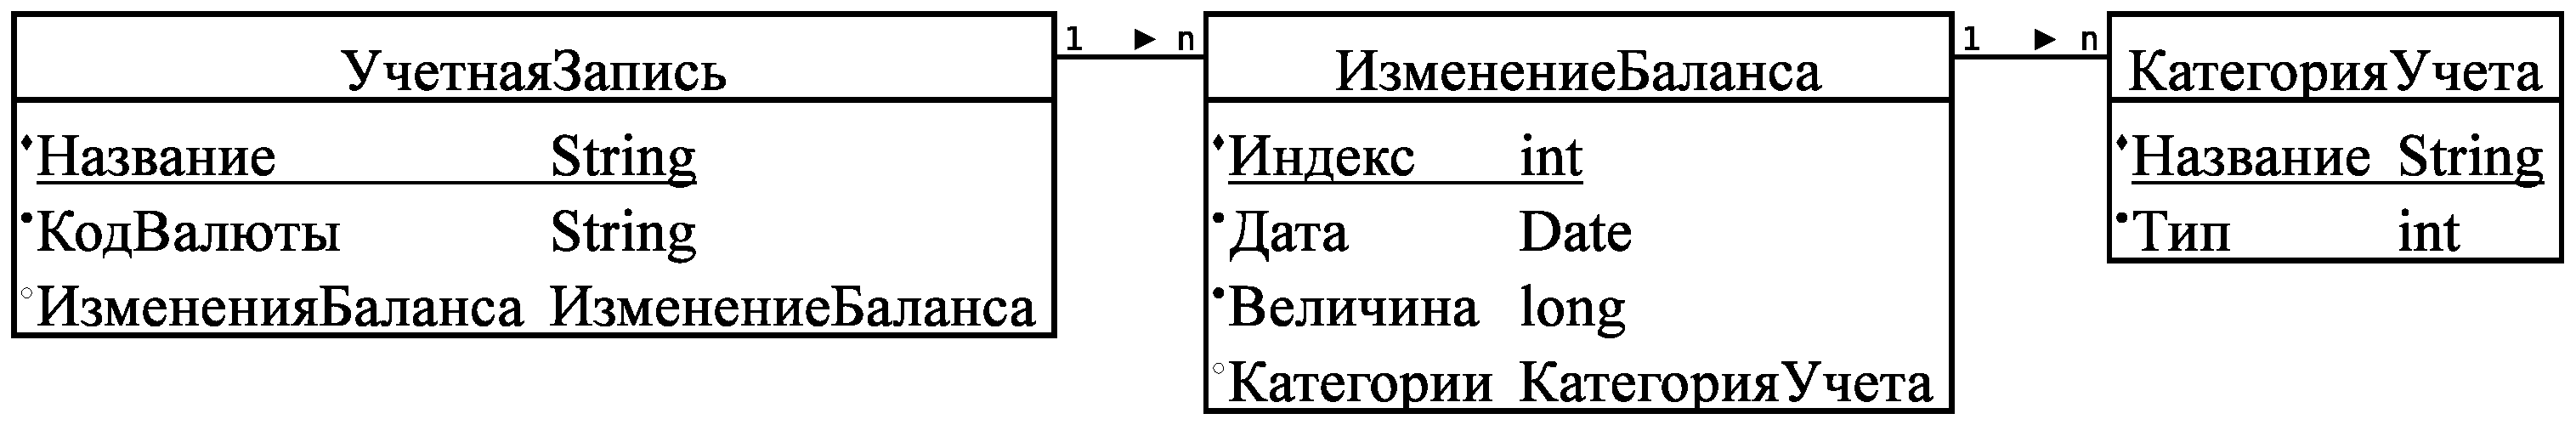
\includegraphics[width=140mm]{fig/design_entities.eps}
  }
  \caption{Модель данных приложения}
  \label{fig:design_entities}
\end{figure}

В соответствии с ней, сущность <<УчетнаяЗапись>> имеет поле названия,
являющееся ключевым, поле кода валюты, соответсвующее коду валюты по
стандарту ISO 4217, а также ссылку на множество сущностей
<<ИзменениеБаланса>>. Данные сущности имеют служебное поле <<Индекс>>,
являющееся ключевым, поле даты регистрации, величины изменения баланса,
а также ссылку на множество связанных категорий.
Сущность <<Категория>> имеет ключевое поле названия, а также поле типа,
определяющее, относится ли данная категория к доходам или расходам.

Определенный интерес представляет вопрос выбора типа данных для хранения
значения изменения баланса. Дело в том, что для хранения финансовых данных
использовать дробные типы данных не рекомендуется
из-за ошибок округления~\cite{bloch08}. С другой стороны, не все СУБД
поддерживают специализированный тип данных для работы с валютой.
В связи с этим для хранения финансовой информации используется целочисленное
поле двойной длины (\texttt{long}), младшие девять разрядов которого используются
для хранения дробной части, а старшие --- для хранения целой части
исходной величины.

Ввод данных в приложение носит преимущественно ручной характер:
например, при вводе данных об изменении баланса
пользователь приложения должен ввести величину изменения баланса,
выбрать желаемые категории и указать дату.
Использование экспериментальной подсистемы OCR позволяет производить
ввод данных о величине изменения баланса в полуавтоматическом режиме.
Вывод данных производится в текстовом и графическом виде и
представляет как собственно хранимые данные, так и данные, полученные путем
применения агрегатных функций. Например, практический интерес представляют
суммы изменений баланса за указанный период, а также распределение
данных сумм по различным категориям учета.

% \subsection{Математическое обеспечение}

% Этапы процесса распознавания образов.
% Краткое математическое описание алгоримов, используемых на каждом этапе.
% Достоинства/недостатки/мотивация выбора.

% \subsection{Алгоритмическое обеспечение}

% % Проектирование алгоритма распознавания изображений.
% % Блок-схема окончательного алгоритма распознавания.

\subsection{Системные требования}

Разрабатываемое приложение предназначено для работы на мобильных устройствах
под управлением операционной системы Android версии не ниже 4.0.x (android-15).
Целевое устройство должно иметь ARM-совместимый процессор с тактовой частотой не менее
1 ГГц и располагать оперативной памятью объемом не менее 128 MБ.
Для полноценной работы приложения требуется наличие фотокамеры,
расположенной на тыльной стороне устройства.

\subsection{Эргономическое обеспечение}

В данном подразделе рассматриваются общие вопросы оформления
пользовательского интерфейса приложения.
Логика связей различных экранов описывается в подразделе~\ref{subsec:design_structure},
а прочие детали реализации пользовательского интерфейса рассматриваются в
подразделе~\ref{subsec:implementation_ui}.

В течение достаточно долгого времени внешний вид пользовательского интерфейса
приложений под управлением платформы Android не был регламентирован:
внешний вид, размещение и шаблоны взаимодействия различных элементов управления
были отданы на откуп разработчикам приложения.
Как следствие, внешний вид различных приложений мог принципиально различаться.
Эта особенность представляла собой существенный недостаток платформы
с точки зрения пользователя.
В 2014 году компания Google представила сообществу Material Design ---
свод рекомендаций по оформлению элементов пользовательского интерфейса
мобильных приложений. Вместе с публикацией этих рекомендаций были
разработан набор библиотек, позволяющих применить данные рекомендации
на предыдущие версии платформы.
Данный свод рекомендаций находится в открытом доступе в сети
Интернет~\cite{material_design}.
В настоящее время подавляющее большинство приложений разрабатывается
в соответствии с ним.

Material design вводит ключевое понятие материала в контексте
пользовательского интерфейса приложения и рассматривает следующие
особенности его использования:
\begin{itemize}
\item дает общие рекомендации об эффективной организации интерфейса
  в виде паттернов поведения;
\item описывает использование наборов цветов, иконок и шрифтов;
\item регламентирует использование теней и отступов,
  а также анимации для переходов между различными состояниями;
\item приводит конкретные примеры оформления элементов
  пользовательского интерфейса.
\end{itemize}
В целом, использование данного документа существенно упрощает процесс
проектирования пользовательского интефейса.

На рисунке~\ref{fig:design_colors} представлена цветовая палитра
разрабатываемого приложения. Цвета <<Индиго>> и <<Темно-голубой>>
используются в качестве основных элементов интерфейса:
панели навигации, панелей выбора вкладок.

\begin{figure}[h!]
  \centering
  \fcolorbox{gray}{white}{
    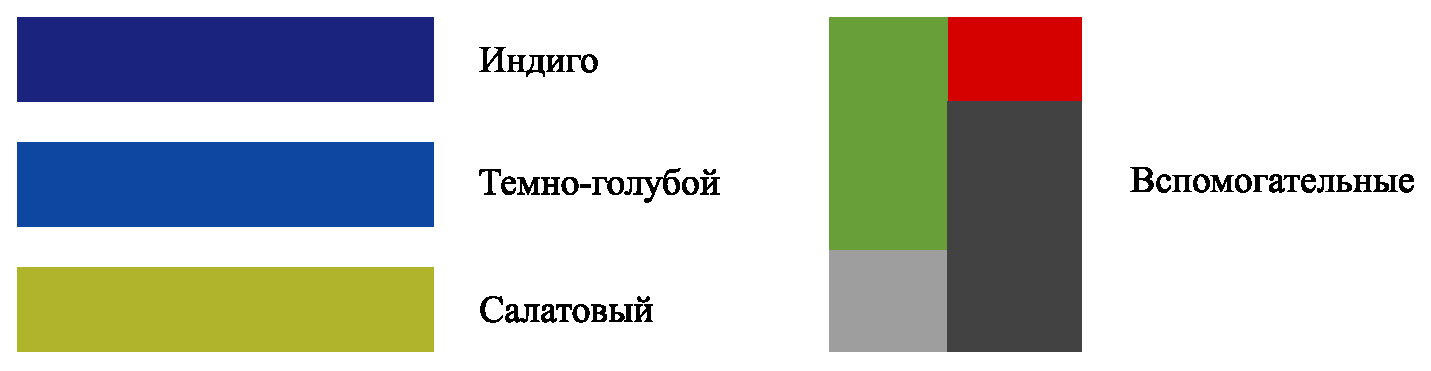
\includegraphics[width=140mm]{fig/design_colors.eps}
  }
  \caption{Используемая цветовая палитра}
  \label{fig:design_colors}
\end{figure}

Салатовый цвет используется для подсвечивания выбранных вкладок,
а также выделения активных полей ввода.
Вспомогательные цвета используются в качестве фоновых цветов списков,
а также для оформления текста.

Material design предписывает использование семейства шрифтов
Roboto sans для отображения текста, состоящего из латинских,
а также клириллических символов. Кроме этого, он регламентирует
использование различных размеров и начертаний данного шрифта.
Правилом хорошего тона является использование не более трех
различных начертаний шрифта на одном экране.
На рисунке~\ref{fig:design_fonts} приведен набор
шрифтовых начертаний, используемых в приложении.

\begin{figure}[h!]
  \centering
  \fcolorbox{gray}{white}{
    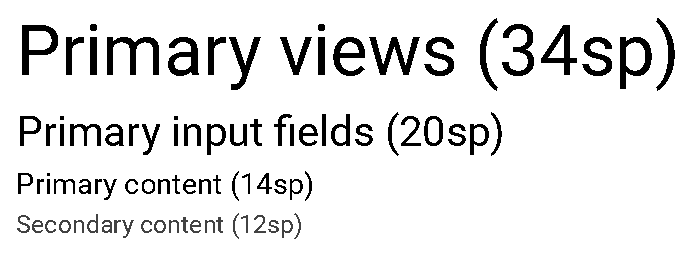
\includegraphics[width=140mm]{fig/design_fonts.eps}
  }
  \caption{Используемый набор начертаний}
  \label{fig:design_fonts}
\end{figure}

Все эти начертания основаны на базовом начертании шрифта Roboto Sans.
Размер начертаний указан в scale-independent pixels, учитывающих различия
в размерах и плотности дисплеев различных целевых устройств,
а также параметров настройки операционной системы.
Шрифт размером в 34sp применяется для отображения в первую очередь
текущего состояния счетов пользователя;
размер в 20sp используется при заполнении обязательных полей при вводе данных;
размеры 14sp и 12sp --- для отображения основного и вспомогательного текста
соответственно.

Кроме этого, разрабатываемое приложение использует иконки для
наглядного представления доступных пользователю опций меню.
Все они являются векторными изображениями, источником для них
является соответствующий репозиторий иконок Material Design.